\documentclass[../main]{subfiles}
\begin{document}

\chapter{Linear Regression}
\begin{introduction}
\item ERM
\item Gradient Descent
\item Ridge Regression ($L_2$ regularization)
\item Lasso Regression ($L_1$ regularization)
\end{introduction}
\section{Basic Knowledge}
\begin{example}
\textbf{Linear Regression}
\end{example}

{Settings.}
\begin{itemize}
  \item Dataset: $D=\{(x_i,y_i)\}_{i=1}^n$, where $x_i\in\mathbb{R}^d$ and $y_i\in\mathbb{R}$.  
  Here, $y_i$ denotes the regression target, while $x_i$ represents the input features used to predict $y_i$.

  \item Linear Model: $f(x)=W^{\top}x+b$, with weight $W\in\mathbb{R}^d$ and bias $b\in\mathbb{R}$.  
  \begin{note}
    This definition is equivalent to an inner product:  
    $\hat y = W^{\top}x+b.$
  \end{note}

  \begin{definition}[Learnable / Trainable Parameters]
    Learnable parameters are those that can be updated during the training process.
  \end{definition}
\end{itemize}

\textbf{Quiz.} How to determine whether a parameter is learnable?
Quiz: How to determine $W$ and $b$?

\noindent Ans: \textbf{ERM} (Empirical Risk Minimization)

\begin{itemize}
  \item Loss function. Squared Loss (SE) is commonly used during optimization. The training objective can be written as:
    \begin{equation}
        \argmin_{W,b}{\color{blue}{\frac{1}{n}}}\sum_{i\in[n]}\left(y_i-(W^\top x_i+b)\right)^2
      \end{equation}
  
  The blue factor $1/n$ can be omitted in theoretical analysis, but is often kept in practice to stabilize the loss function during implementation.
\end{itemize}
Quiz: How to optimize the parameters?

\noindent Ans: \textbf{Gradient Descent} (as a traditional ML method). In the case of linear regression:
\begin{gather}
  \frac{\partial \mathcal L}{\partial b}=-2\sum_{i\in[n]}(y_i-W^\top x_i-b)\\
  \frac{\partial \mathcal L}{\partial W}=-2\sum_{i\in[n]}(y_i-W^\top x_i-b)x_i
\end{gather}
\begin{note}
  In the field of machine learning, the gradient of a scalar with respect to a vector is itself a vector \textbf{(not a covector)}. This means:
  \begin{equation}
    \frac{\partial \mathcal L}{\partial W}=\begin{pmatrix}
      \frac{\partial \mathcal L}{\partial W_1}\\
      \frac{\partial \mathcal L}{\partial W_2}\\
      \vdots\\
      \frac{\partial \mathcal L}{\partial W_d}
    \end{pmatrix}=\left(\frac{\partial \mathcal L}{\partial W_1},
    \frac{\partial \mathcal L}{\partial W_2},
    \cdots,
    \frac{\partial \mathcal L}{\partial W_d}\right)^\top
  \end{equation}
\end{note}
\begin{note}
  Here are some commonly used derivative formulas:
  \begin{gather}
    \frac{\partial x^\top x}{\partial x}=2x\\
    \frac{\partial a^\top x}{\partial x}=a,\quad \frac{\partial Ax}{\partial x}=A^\top\\
    \frac{\partial x^\top Ax}{\partial x}=(A+A^\top)x
  \end{gather}
\end{note}
\begin{remark}
  Both sides of an equation must have the same dimension. This principle can be used as a consistency check.
\end{remark}
We optimize the parameters by subtracting a scalar multiple of the gradient from the parameters, considering the physical meaning of the gradient: the direction of the steepest \textbf{increase}.
\begin{definition}[Hyperparameter]
    A parameter that is fixed during optimization and specified before the training process.
\end{definition} 
That is:
\begin{equation}
    W'=W-\alpha\frac{\partial\mathcal L}{\partial W },\quad b'=b-\alpha\frac{\partial \mathcal L}{\partial b}
\end{equation}
Optimization will stop when the norm of the parameter update becomes smaller than a given hyperparameter.
\section{Closed-Form of Linear Regression}
\begin{proposition}
  Linear Regression has \textbf{Closed-Form} solution.
\end{proposition}
Settings.
\begin{itemize}
  \item Metrix $X_0:=(x_1^\top,\cdots,x_n^{\top})^\top$ ; 
  \item Metrix $X:=(X_0,\mathbb 1)\in \mathbb R^{n\times(d+1)}$;
  \item $y=(y_1,\cdots,y_n)^\top\in\mathbb R^n$;
  \item $\hat w=(w,b)^\top\in\mathbb R^{d+1}$.
\end{itemize}
Then the loss function of $\hat w$ can be writtern as:
\begin{equation}
    \mathcal L(\hat w)=(y-X\hat w)^\top (y-X\hat w)=\|y-X\hat w\|_2^2
\end{equation}
Here, $\|\cdot\|_p$ denotes the \emph{p-norm} of a vector.
\begin{note}
  Vectors can sometimes be treated as scalars, since linearity ensures that the validity of a proposition can be extended to any finite dimension.  
\end{note}
Notice that the optimization stops when $\partial\mathcal L(\hat w)/\partial \hat w=0$. Under this condition, the parameters can be solved from the above constraint by following steps:
\begin{align}
  \frac{\partial\mathcal L(\hat w)}{\partial\hat w}&=-2X^\top(y-X\hat w)
\end{align}
\begin{note}
  Both dimensional analysis and calculation using Leibniz's rule lead to the same result as the formula above:
  \begin{align*}
      \mathcal L(\hat w)&=y^\top y-2y^\top X\hat w+\hat w^\top X^\top X\hat w\\
      \partial_{\hat w}\mathcal L(\hat w)&=-2X^\top y+2X^\top X\hat w\\
      &=-2 X^\top(y-X\hat w)
  \end{align*}
\end{note}
\begin{remark}
  More matix formulas are available in \href{https://www.math.uwaterloo.ca/~hwolkowi/matrixcookbook.pdf}{Matrix Cookbook}.
\end{remark}
Thus, the target of the optimization satisfied:
\begin{equation}
    X^\top y=X^\top X\hat w
\end{equation}
That is:
\begin{equation}
    \hat w=(X^\top X)^{-1}X^\top y
\end{equation}
when $X^\top X$ invertible (non-singular / full-rank).
\begin{example}
  When does $X^\top X$ not invertible?
\end{example}
\begin{solution}
  $X\in \mathbb R^{n\times(d+1)}$:
\begin{itemize}
  \item $d+1>n.$ Brief Proof: $\, \rank (X^\top X)=\rank (X)\le\min(n,d+1)=n<d+1$.
  \item $X$ has repeated columns. Proof is trivial.
\end{itemize}
\end{solution}

\vspace{1em}
When $X^\top X$ isn't invertible:
\begin{enumerate}
  \item If $\rank (X^\top X, X^\top y)>\rank (X^\top X)$, $\hat w$ has no solution; 
  \item $\hat w$ has infinity solution o.w.
\end{enumerate}
Situation 1 is \textbf{Impossible} because both $X^\top X$ and $X^\top y$ can be represented in the column space of $X^\top$. Therefore, the optimization problem must have a solution, which may be either unique or infinite.

As an infinite set of solutions makes it difficult to determine which estimate of $\hat w$ to choose, we apply \textbf{$L_2$ regularization} to linear regression, which is commonly referred to as \textbf{Ridge Regression}. That is:
\begin{equation}
    \mathcal L_{L_2}:=\mathcal L(\hat w)+\boxed{\lambda\|\hat w\|_2^2}
\end{equation}
Noticed that $\|\hat w\|_2^2=\sum_{i=1}^{d+1}\hat w_i^2$, $L_2$ regularization prevents any single dimension from being assigned an excessively large weight, , and encourages the model to make use of more dimensions during training.
\begin{figure}[H]
  \centering
  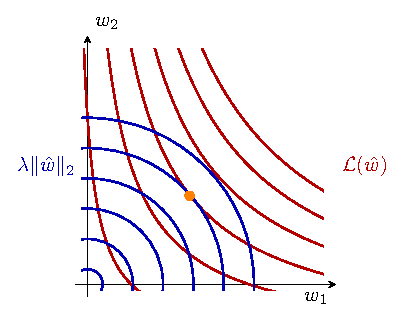
\includegraphics{../../tikz/1/2-2.pdf}
  \caption{Illustration of $L_2$ regularization. 
The contours represent level sets of the regularized loss $\mathcal{L}(\hat w) + \lambda \|\hat w\|_2^2$, 
which take the form of concentric ellipses (circle in the plot). }
\end{figure}

During ridge regression, we minimize the $\mathcal L_{L_2}$:
\begin{equation}
    \argmin_{\hat w}\,(y-X\hat w)^\top(y-X\hat w)+\lambda\hat W^\top \hat W
\end{equation}
The optimization stops when:
\begin{align}
  \frac{\partial \mathcal L_{L_2}}{\partial \hat w}&=-2X^\top y+2X^\top X\hat w+2\lambda I\hat w=0\\
  &\Rightarrow (X^\top X+\lambda\mathbb I)\hat w=X^\top w
\end{align} 
\begin{proposition}
$X^\top X+\lambda\mathbb I$ always invertible.
\end{proposition}
\begin{proof}
  Since $X^\top X$ is a real symmetric matrix, we have the eigen-decomposition
  $X^\top X=U\Lambda U^\top$, where $\Lambda=\mathrm{diag}(\lambda_1,\cdots,\lambda_{d+1})$.  
  Moreover, as $X^\top X\succeq 0$ is positive semi-definite, it follows that $\forall i\in [d+1],\,\lambda_i\ge 0$.  
  Note that:
  \begin{equation}
      \lambda\mathbb I=\lambda UU^\top
  \end{equation}
  since $U$ is an orthogonal matrix. Hence:
  \begin{equation}
      X^\top X+\lambda\mathbb I=U(\Lambda+\lambda I)U^\top
  \end{equation}
  For all $i\in[d+1]$, we have:
  \begin{equation}
      \lambda_i+\lambda>\lambda_i\ge 0 
  \end{equation}
  Thus, $X^\top X+\lambda I$ is a full-rank matrix.
\end{proof}
\begin{remark}
  Numerical issues may still occur even if $X^\top X$ is full rank (e.g., when eigenvalues $\lambda_k$ are close to zero).  
  The $L_2$ regularization factor $\lambda$ mitigates this issue by shifting the eigenvalues upward, thereby improving numerical stability during training.
\end{remark}

Another regularization method often used is $L_1$ regularization, where the loss function is defined as:
\begin{equation}
    \mathcal L_{L_1}:=\mathcal L(\hat w)+\boxed{\lambda\|\hat w\|_1}
\end{equation}
$L_1$ regularization can induce sparsity in $\hat w$, which works in contrast to $L_2$ regularization.  
Specifically, $L_1$ regularization encourages the model to rely on only a small subset of input features, effectively performing \textbf{feature selection}.

Linear regression with $L_1$ regularization is called \textbf{Lasso Regression} (Least Absolute Shrinkage and Selection Operator).
\begin{figure}[H]
  \centering
  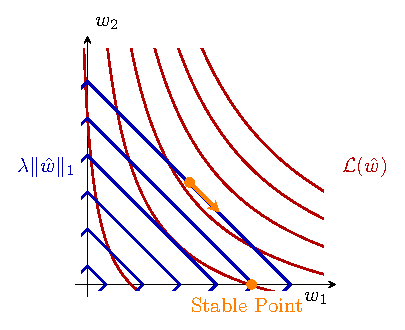
\includegraphics{../../tikz/1/2.pdf}
  \caption{Illustration of $L_1$ regularization. 
  The contours represent level sets of the regularized loss $\mathcal{L}(\hat w) + \lambda \|\hat w\|_1$, 
  which take the form of nested diamonds (squares rotated by $45^\circ$ in the plot). }
\end{figure}
\section{Geomeric View of LR}

Ideally, we would like to solve $X \hat w = y.$ If $y$ lies on the hypersurface 
\begin{equation}
  \mathcal{M}(X) :=\mathrm{Span}(X)= \{ X w : w \in \mathbb{R}^d \} \subset \mathbb{R}^n
\end{equation}
then the equation admits an exact solution. In most cases, however, $y \notin \mathcal{M}(X)$, so no exact solution exists. Nevertheless, we can always find an estimator $\hat w$ such that $\mathcal P_{\mathcal{M}(X)} y = X \hat w$, where $\mathcal P_{\mathcal{M}(X)}$ denotes the orthogonal projection onto the hypersurface $\mathcal{M}(X)$.
\begin{proposition}
  \begin{equation}
      \hat y=X\hat w\quad\Rightarrow\quad\hat w \text{ is solution to LR.}
  \end{equation}
\end{proposition}
\begin{proof}
  \begin{align*}
    y-\hat y\,\bot\, \mathcal{M}(X)\quad&\Rightarrow\quad y-X\hat w\,\bot\, \mathcal{M}(X)\\
    &\Rightarrow\quad X^\top(y-X\hat w)=0\quad\Rightarrow\quad \hat w=(X^\top X)^{-1}X^{\top}y
  \end{align*}
\end{proof}
\begin{figure}[H]
  \centering
  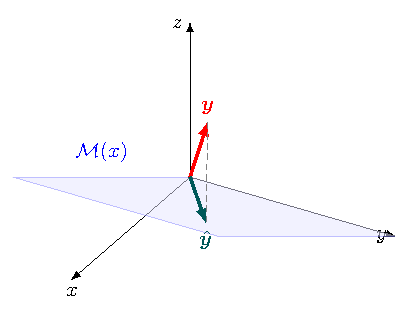
\includegraphics{../../tikz/1/3.pdf}
  \caption{Orthogonal projection interpretation of linear regression. 
The predicted vector $X\hat w$ is obtained as the projection of $y$ onto the hypersurface 
$\mathcal M(X)=\{Xw : w\in\mathbb{R}^d\}$, which is a linear subspace in the classical case.}
\end{figure}

\end{document}